\section{Descrição e exploração dos datasets}

\subsection{Previsão do número de incidentes rodoviários}
Dataset relativo ao número de incidentes rodoviários na cidade de Braga.
Possui as seguintes features: 
\begin{itemize}
    \item \textbf{city\_name} - nome da cidade, no caso dos registos utilizados tem sempre o valor "Braga";
    \item \textbf{record\_date} - data em que o registo foi efetuado;
    \item \textbf{magnitude\_of\_delay} - magnitude do atraso provocado pelos incidentes referentes ao registo em causa;
    \item \textbf{delay\_in\_seconds} - atraso, em segundos, provocado pelos incidentes que se verificam no registo;
    \item \textbf{affected\_roads} - estradas afectadas pelos incidentes para cada registo;
    \item \textbf{luminosity} - o nível de luminosidade que se verificava na cidade de Braga;
    \item \textbf{avg\_temperature} - valor médio da temperatura na cidade de Braga no momento em que o registo foi efetuado;
    \item \textbf{avg\_atm\_pressure} - valor médio da pressão na cidade de Braga no momento em que o registo foi efetuado;
    \item \textbf{avg\_humidity} - valor médio da humidade na cidade de Braga no momento em que o registo foi efetuado;
    \item \textbf{avg\_wind\_speed} - valor médio da velocidade do vento na cidade de Braga no momento em que o registo foi efetuado;
    \item \textbf{avg\_precipitation} - valor médio de precipitação na cidade de Braga no momento em que o registo foi efetuado;
    \item \textbf{avg\_rain} - avaliação qualitativa do nível de precipitação para o record\_date na cidade de Braga;
    \item \textbf{accidents} - indicação acerca do nível de incidentes rodoviários que se verificam no record\_date correspondente na cidade de Braga.
\end{itemize}

Após uma preparação dos dados foram removidos alguns parâmetros e criados outros, assim sendo, do dataset original foram removidas as colunas \textbf{"city name"}, \textbf{"avg\_atm\_pressure"}, \textbf{"avg\_precipitation"} e \textbf{"avg\_rain"}. Através de \textit{Feature Engineering} conseguimos extrair dados adicionais de algumas outras colunas. No caso, \textbf{record\_date} subdividiu-se em \textbf{Month}, \textbf{Day of year}, \textbf{Day of week} e \textbf{Hour}. 



A coluna \textbf{affected\_roads} foi utilizada para calcular o numero de incidentes ativos no momento do registo. No entanto, denotamos que o número de elementos calculados pelo atributos \textbf{affected\_roads} não é diretamente correspondente ao número de acidentes real à data daquele registo, por meio de análise dos dados descobrimos que podem existir estradas repetidas nesse atributo, sem que tenha existindo mais do que um acidente nessa mesma estrada, este caso poderá representar, na realidade, acidentes cuja magnitude seja tamanha que implicou o registo do mesmo acidente várias vezes ao longo do dia. Inicialmente, ponderou-se que este atributo pode-se estar relacionado com o atributo de \textit{delay} em segundos. Terá sido teorizado, que, de determinada forma, quanto maior fosse o número de acidentes maior seria a probabilidade de existir registos repetidos do mesmo acidente numa dada estrada, sem que tenha existindo mais do que um acidente nessa mesma estrada. No entanto, não foi possível chegar a uma conclusão imediata sobre esta relação de \textit{delay} em segundos e número de acidentes repetidos.


    \begin{figure}[H]
        \centering
        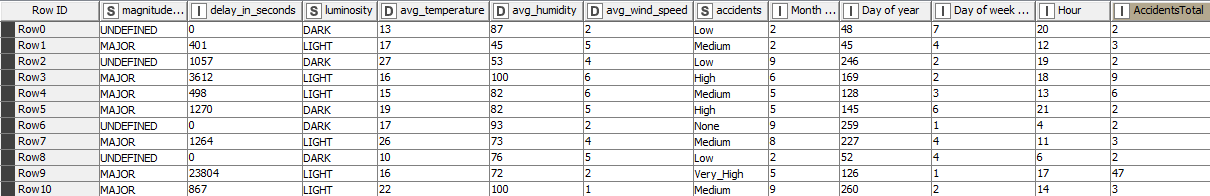
\includegraphics[width=0.8\linewidth]{Figures/excerto_dataset_braga.png}
        \caption{Segmento do dados de treino, após pré-processamento.}
        \label{fig:"um"}
    \end{figure} 

\subsection{League of Legends - previsão baseada nos 10 primeiros minutos de jogo}
O dataset utilizado neste ponto continha inicialmente 39, algumas delas redundantes. Assim sendo não será explicado de forma detalhada a constituição do dataset inicial. No entanto, mais adiante será explicado qual o processo utilizado para decidirmos quais deveriamos remover.

Assim sendo, o dataset final possui os seguintes campos:
\begin{itemize}
    \item \textbf{blueWins} - Valor indicativo de qual equipa obteve venceu, se o valor for "1" indica que foi a equipa azul, caso contrário terá sido a equipa vermelha.
    \item \textbf{blueFirstBlood} - Valor indicativo de qual equipa obteve \gls{firstBlood}, se o valor for "1" indica que foi a equipa azul, caso contrário terá sido a equipa vermelha
    \item \textbf{diffWardsPlaced} - diferença entre o número de \gls{wards} colocados em campo pela equipa azul e pela vermelha.
    \item \textbf{diffWardsDestroyed} - diferença entre o número de \gls{wards} destruidos pela equipa azul e pela vermelha.
    \item \textbf{diffKills} - diferença entre o número de \gls{kills} da equipa azul e da equipa vermelha
    \item \textbf{diffAssists} - diferença entre o número de \gls{assists} da equipa azul e da equipa vermelha
    \item \textbf{diffEliteMonsters} - diferença entre o número de \gls{eliteMonster} mortos pelas equipas.
    \item \textbf{diffDragons} - diferença entre o número de \gls{dragons} mortos pelas equipas.
    \item \textbf{diffHeralds} - diferença entre o número de \gls{heralds} mortos pelas equipas.
    \item \textbf{diffTowersDestroyed} - diferença entre o número de \gls{torres} destruidas por cada equipa
    \item \textbf{diffTotalGold} - diferença entre a quantidade de \gls{gold} de cada equipa.
    \item \textbf{diffTotalExperience} - diferença entre o nível de \gls{experiencia} de cada equipa.
    \item \textbf{diffTotalMinionsKilled} - diferença entre a quantidade de \gls{minions} mortos por cada equipa.
    \item \textbf{diffTotalJungleMinionsKilled} - diferença entre a quantidade de \gls{jungleMinions} mortos por cada equipa.
    \item \textbf{diffAvgLevel} - diferença entre o \gls{nivel} médio de cada equipa.
\end{itemize}